%%%%%%%%%%%%%%%%%%%%%%%%%%%%%%%%%%%%%%%%%
% Simple Sectioned Essay Template
% LaTeX Template
%
% This template has been downloaded from:
% http://www.latextemplates.com
%
% Note:
% The \lipsum[#] commands throughout this template generate dummy text
% to fill the template out. These commands should all be removed when 
% writing essay content.
%
%%%%%%%%%%%%%%%%%%%%%%%%%%%%%%%%%%%%%%%%%

%----------------------------------------------------------------------------------------
%	PACKAGES AND OTHER DOCUMENT CONFIGURATIONS
%----------------------------------------------------------------------------------------

\documentclass[12pt]{article} % Default font size is 12pt, it can be changed here

\usepackage{geometry} % Required to change the page size to A4
\geometry{a4paper} % Set the page size to be A4 as opposed to the default US Letter

\usepackage{graphicx} % Required for including pictures

\usepackage{float} % Allows putting an [H] in \begin{figure} to specify the exact location of the figure


\usepackage{lipsum} % Used for inserting dummy 'Lorem ipsum' text into the template

\linespread{1.2} % Line spacing

%\setlength\parindent{0pt} % Uncomment to remove all indentation from paragraphs

\graphicspath{{Pictures/}} % Specifies the directory where pictures are stored

\begin{document}

%----------------------------------------------------------------------------------------
%	TITLE PAGE
%----------------------------------------------------------------------------------------

\begin{titlepage}

\newcommand{\HRule}{\rule{\linewidth}{0.5mm}} % Defines a new command for the horizontal lines, change thickness here

\center % Center everything on the page

\textsc{\LARGE Politecnico di Milano}\\[1.5cm] % Name of your university/college
\textsc{\Large Dipartimento di elettronica, informazione e bioingegneria}\\[0.5cm] % Major heading such as course name
\textsc{\large Image analysis}\\[0.5cm] % Minor heading such as course title

\HRule \\[0.4cm]
{ \huge \textbf{ Software for traffic violation of 
\\ a right hand rule}}\\[0.4cm] % Title of your document
\HRule \\[1.5cm]

\begin{minipage}{0.4\textwidth}
\begin{flushleft} \large
\emph{Author:}\\
Mirjam \textsc{Skarica},\\ 
Lucija \textsc{Megla} % Your name
\end{flushleft}
\end{minipage}
~
\begin{minipage}{0.4\textwidth}
\begin{flushright} \large
\emph{Supervisor:} \\
prof. Vincenzo \textsc{Caglioti} % Supervisor's Name
\end{flushright}
\end{minipage}\\[4cm]

{\large \today}\\[3cm] % Date, change the \today to a set date if you want to be precise

%\includegraphics{Logo}\\[1cm] % Include a department/university logo - this will require the graphicx package

\vfill % Fill the rest of the page with whitespace

\end{titlepage}

%----------------------------------------------------------------------------------------
%	TABLE OF CONTENTS
%----------------------------------------------------------------------------------------

\tableofcontents % Include a table of contents

\newpage % Begins the essay on a new page instead of on the same page as the table of contents 

%----------------------------------------------------------------------------------------
%	INTRODUCTION
%----------------------------------------------------------------------------------------

\section{Introduction} % Major section

In the last few decades there has been a huge growth of traffic in the big cities. In consequence with growth of traffic, number of violations increased. As a result, software for traffic violation detection is a way to maintain order and track violations in a profitable way.

%------------------------------------------------

\subsection{Motivation and formulation of the problem} % Sub-section

Even though many crossroads have traffic lights or traffic signs, there are still crossroads without any of it. As many know, in that particular case right-hand rule is applied. In absence of traffic lights or signs, right hand rule demands from a driver of a vehicle to give away the priority to vehicles approaching from the right at intersections.

Given the above problem, the goal of the project is to develop a software that is going to recognize violations of the right hand rule and inform the operator about it. This way, we could gain an automated way to recognize this type of violations, which could help track situations on every intersection without traffic lights or signs. This is going to make tracking of right hand rule violations far more easier and profitable.

%------------------------------------------------

\subsection{Camera and acquisition of video material} % Sub-section

Formulation of the project for developing software for right-hand rule violations guarantees acquisition of the video material through a traffic surveillance camera placed in an elevated area. 
Since we did not have a surveillance camera at our disposal, we used a classical digital camera attached to an elevated object. Our camera had a frame rate of 30 fps and was attached to a trivet to reduce vibrations and other disturbances in order to capture a credible situation.



%------------------------------------------------

\subsection{Document structure}

This document serves to describe the structure of the software and its implementation in detail. Also, a detailed utility manual is given to describe software use-cases and to give a glimpse of situations in which software will work and some situations in which might fail.
\\

The report is divided into two sections:
\begin{enumerate}
\item Structure of the software and its implementation, in which we describe in detail approached used in development of our software;
\item Results, in which we give a critical review of our software and we list possible improvements of it. 
\end{enumerate}

%------------------------------------------------


%----------------------------------------------------------------------------------------
%	MAJOR SECTION 1
%----------------------------------------------------------------------------------------

\section{Structure of the software and its implementation} % Major section

To get a software that recognizes traffic violations of a right hand rule, we had to divide the task in more subtasks to get the desired behaviour. Those subtasks can be seen in Figure \ref{fig:workflow}.

\begin{figure}[ht]
\centering
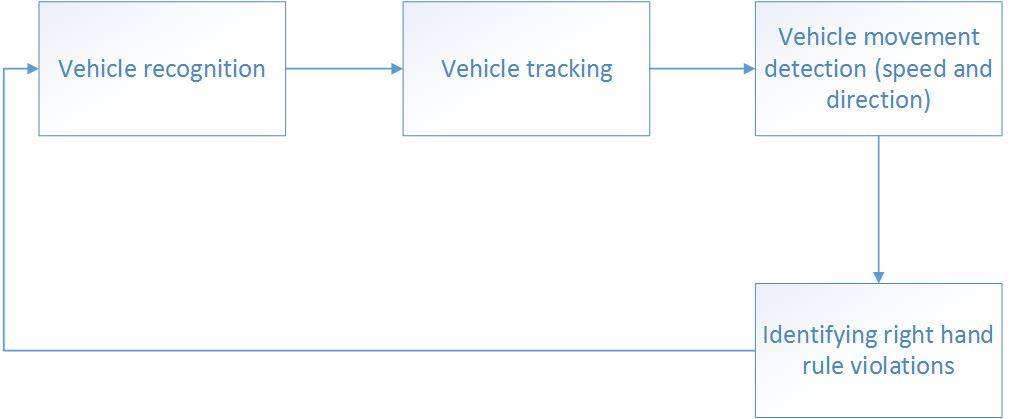
\includegraphics[width=10cm]{Drawing1.jpg}
\caption{Software workflow}
\label{fig:workflow}
\end{figure}

As we can see from Figure 1., first step in our algorithm consist of car recognition. In this step we had to extract background from the foreground and recognize cars in the given foreground. After extracting vehicles from the video footage, we had to track them through frames, so that we could determine their speed and direction. To identify if there is a violation of the right hand rule in the intersection, we divided the intersection in priorities and with the help of car's direction and speed determined if the violation occurred or not.

%------------------------------------------------

\subsection{Vehicle recognition} % Sub-section

When we look at problems video surveillance could solve, we need to make sure the system is robust. To say the system of video surveillance is robust, it should not depend on correct position of the camera and it should not lose its performance when there are:

\begin{itemize}
\item objects that can be partially seen in the scene
\item overlapping objects in the scene
\item shadows
\item changes of lightning
\item objects that move slowly
\item objects that were visible and then removed from the scene
\end{itemize}

Talking about recognizing of vehicles, the problem of their identification consists mostly of being able to keep good estimation of the foreground. After that, applying filters to foreground estimation will give us a foreground with more quality in which we can extract vehicles with \textit{blob analysis}.
In the next few paragraphs we are going to explain all three steps in detail.

\subsubsection{Foreground estimation}

Major part of foreground estimation approaches are based on background estimation, which do not apply on our problem, that is, they did not give good results. That is why we chose to work with Gaussian Mixture Models (GMM), which gave us flexibility and robustness to confront all the problems stated above. Although different methods of GMM exist, like the one of Friedman and Russell ([FR97]), which explicitly classifies values of pixels with three different distributions and determines if the pixels belong to the street, shadows or vehicles, the method implemented in our software is the one of Stauffer and Grimson [SG99]. This method of GMM does not model all the pixels with one particular distribution, but models the value of one pixel with mixture of different Gaussians; the motive for using mixture of different Gaussians lies in the fact that  multiple surfaces often appear in the view frustum of a particular pixel and the lighting conditions change. Hence, mixture of Gaussians is able to surpass those changes. Each time the parameters of the Gaussians are updated,
the Gaussians are evaluated using a simple
heuristic to hypothesize which are most likely to be part of the "background process". Pixel values that do not match one of the pixel’s "background" Gaussians are grouped using connected components. Finally, the connected components are tracked from frame to frame using a multiple hypothesis tracker. 
This method uses two parameters: $\alpha$ and $T$. Parameter $\alpha$ represents learning rate and parameter $T$ is a threshold for determining which distributions belong to the background and which do not.  

We consider the values of a particular pixel over
time as a "pixel process". The "pixel process" is a
time series of pixel values, e.g. scalars for gray values or vectors for color images. At any time $t$, what is known about a particular pixel, ${x_{0}, y_{0}}$, is its history:

\begin{equation}
{\{X_{1},X_{2},...,X_{t}} = {I(x_{0},y_{0},i):1\leq i \leq t\}}
\end{equation}

where $I$ is the image sequence. The recent history of each pixel, ${X_{1}, ..., X_{t}}$, is modeled by a mixture of K Gaussian distributions. The probability of observing the current pixel value is

\begin{equation}
{P(X_{t}) = \sum_{i=1}^{K}\omega_{i,k} \ast \eta(X_{t},\mu_{i,t}, \sum_{i,t})}
\end{equation}

where $K$ is the number of distributions, $\omega_{i,t}$ is an estimate
of the weight (what portion of the data is accounted for by this Gaussian) of the $i$-th Gaussian in the mixture at time $t$, $\mu_{i,t}$ is the mean value of the $i$- th Gaussian in the mixture at time $t$, $\sum_{i,t}$ is the covariance matrix of the $i$-th Gaussian in the mixture at time $t$, and where $\eta$ is a Gaussian probability density function:

\begin{equation}
\eta(X_{t},\mu_{i,t}, \sum_{i,t} = \frac{1}{(2\pi)^{\frac{n}{2}}|\sum|^{\frac{1}{2}}} e^{-\frac{1}{2}(X_{t}-\mu_{t})^{T}\sum^{-1}(X_{t}-\mu_{t})}
\end{equation}

K can take values between 3 and 5. In this case, 5 is used. Also, for computational reasons, the covariance matrix is assumed to be of the form:

\begin{equation}
{\sum_{k,t} = \sigma_{k}^{2}\textbf{I}}
\end{equation}

This assumes that the red, green, and blue pixel values are independent and have the same variances. While this is certainly not the case, the assumption allows us to avoid a costly matrix inversion at the expense of some accuracy. 
Thus, the distribution of recently observed values
of each pixel in the scene is characterized by a mixture of Gaussians. A new pixel value will, in general, be represented by one of the major components of the mixture model and used to update the model. 

Once we defined the model of the background, it is necessary to initialize diverse parameters of Gaussian mixtures. To avoid costly performance, Stauffer and Grimson [SG99] used K-means algorithm to initialize those parameters. Once we defined those parameters, it is possible to start the foreground estimation. To model this, we need
a method for deciding what portion of the mixture
model best represents background processes. First, the Gaussians are ordered by the value of
${\omega/\sigma}$. This value increases both as a distribution gains more evidence and as the variance decreases. This ordering of the model is effectively an ordered list, where the most likely background distributions remain on top and the less probable transient background distributions gravitate towards the bottom and are eventually replaced by new distributions.

The first $B$ distributions are chosen as background model, where:

\begin{equation}
B = argmin_{b}(\sum_{k=1}^{b}w_{k} > T)
\end{equation}

where $T$ is a measure of the minimum portion of the data that should be accounted for by the background. This takes the "best" distributions until a certain portion $T$, of the recent data has been accounted for. The other distributions are taken as foreground distributions. 
Hence, when a new frame comes in time $t+1$, match test is being held on each pixel; one pixel belongs to a Gaussian distribution if a Mahalanobis (6) inequality is satisfied:

\begin{equation}
sqrt((X_{t+1}-\mu_{i,t})^T\sum_{i,t}^{-1}(X_{t+1}-\mu_{i,t})) < k\sigma_{i,t}
\end{equation}

where $k=2.5$.

With the above equation there are two possible cases:

\begin{enumerate}
\item Pixel and one of $K$ Gaussian distributions were matched. In this case, a pixel is classified as a background pixel if its distribution is marked as a background distribution, or as a foreground pixel otherwise.
\item If we did not find a distribution for a pixel, then the pixel is classified as a foreground pixel.
\end{enumerate}

The result of this procedure on every pixel is a binary matrix which has a value 1 denoting a foreground pixel and a value 0 denoting a background pixel. In Table 1 we can see parameters for foreground estimation used in our software.





\begin{table}
\begin{center}
 \begin{tabular}{||c  c||} 
 \hline
 Name & Value \\ [0.5ex] 
 \hline\hline
 Num. Gaussians & 5  \\ 
 \hline
 Num. frames for learning & 50 \\
 \hline
 T & 0.005 \\
 \hline
 $\alpha$ & 0.2\\
 \hline

\end{tabular}
\end{center}
\caption{Table of parameters for foreground estimation}
\label{table:1}
\end{table}



%------------------------------------------------
\subsubsection{Filter application}

Once we estimated the foreground, it was necessary to apply a filter to remove the noise. First we used function \textit{imopen} which performs morphological opening on the foreground estimation with a square structure element having dimensions $3\times3$. After that we used function \textit{imclose} which performs morphological closing on our estimated foreground. With function \textit{imfill} we performed hole filling on our foreground to get better precision.

In Figure \ref{fig:extr-fg} we can see how the foreground looks like after the extraction and noise removal.

\begin{figure}[ht]
\centering
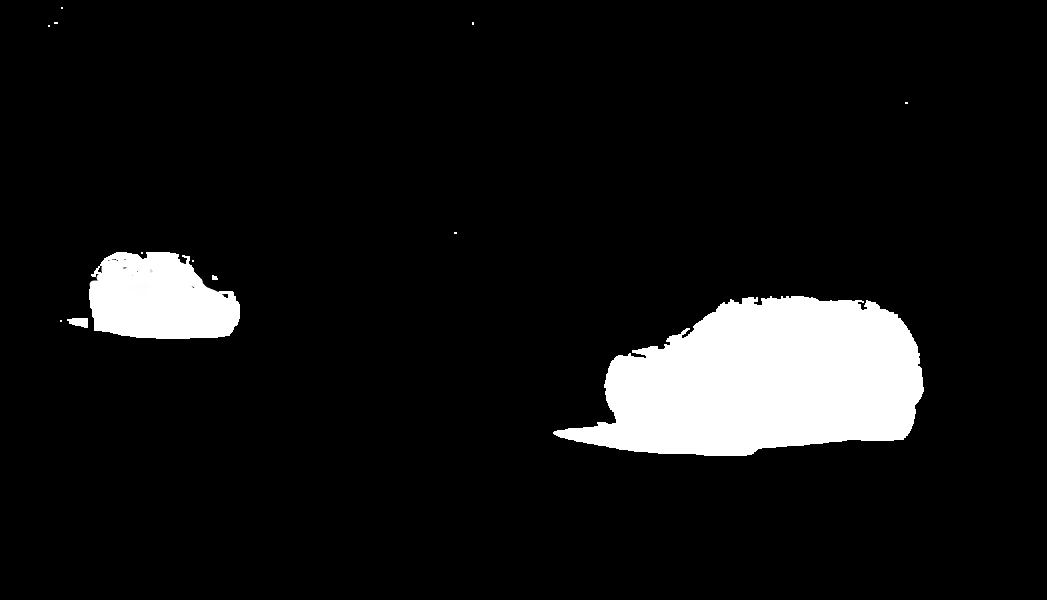
\includegraphics[width=10cm]{images/foreground.png}
\caption{Extracted foreground with noise removed}
\label{fig:extr-fg}
\end{figure}

\subsubsection{Blob analysis}

After extracting the foreground and removing noise, we were ready to extract connected regions as blobs and identify which of the blobs correspond to vehicles. We performed blob analysis with MATLAB's BlobAnalysis. The output of blob analysis contains identified blobs which could correspond to vehicles. To remove possible outliers, we extracted width and hight of the blob and put a constraint over the ratio between the two, which had to be greater than 0.9. If the corresponding blob was detected as a car, we saved its bounding box and centroid.

In Figure \ref{fig:car-detect} we can see how the blobs are represented when processing the videos.
\begin{figure}[ht]
\centering
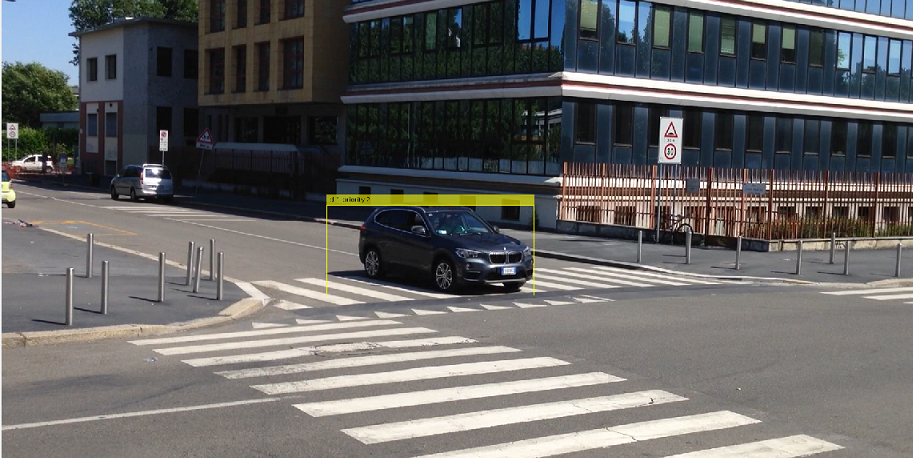
\includegraphics[width=10cm]{images/tracking.png}
\caption{Detecting cars}
\label{fig:car-detect}
\end{figure}

\subsection{Tracking of vehicles}

In order to be able to recognize traffic violations, after foreground detection and blob extraction, we had to be able to track moving vehicles through certain period of time. In this part of our software we were focused strictly on motion.

The problem of motion-based object tracking can be divided into two parts:

\begin{enumerate}
\item detecting moving cars in each frame
\item associating the detections corresponding to the same car object over time
\end{enumerate}

We described detection of moving cars in the previous subsection, where we used a foreground detection algorithm based on Gaussian mixture models, morphological operations to eliminate noise and blob analysis to detect groups of connected pixels, which represented moving vehicles.

The association of detections to the same moving car (i.e track) is based solely on motion. Each track is representing a moving car in the video. The purpose of the structure is to maintain the state of a tracked car. The structure contains the following fields: 
\begin{itemize}
\item id: the integer ID of the track
\item age: the number of frames since the track was first detected
\item bbox: the current bounding box of the object; used for display
\item bbox\_initial: first bounding box
\item velocity: car's speed
\item priority: car's priority; used for violation detection
\item kalmanFilter: a Kalman filter object used for motion-based tracking
\item totalVisibleCount: he total number of frames in which the track was detected (visible)
\item consecutiveInvisibleCount : the number of consecutive frames for which the track was not detected (invisible).
\end{itemize}

The motion of each track is estimated by a Kalman filter. This filter is used to predict the track's location in each frame and determine the likelihood of each detection being assigned to each track.

Track maintenance becomes an important aspect of this example. In any given frame, some detections may be assigned to tracks, while other detections and tracks may remain unassigned. The assigned tracks are updated using the corresponding detections. The unassigned tracks are marked invisible. An unassigned detection begins a new track.

Each track keeps count of the number of consecutive frames, where it remained unassigned. If the count exceeds a specified threshold, the example assumes that the object left the field of view and it deletes the track.

The part of our software which is in charge of tracking moving cars can be divided in several parts:

\begin{itemize}
\item detection of moving cars in the current frame
\item prediction of new locations of existing tracks
\item assignment of detections to tracks
\item update of assigned tracks
\item update of unassigned tracks
\item deletion of lost tracks
\item creation of new tracks
\end{itemize}

For \textit{predicition of new locations of existing tracks} we used Kalman filter. In this section, Kalman filter predicts the centroid of each track in the current frame and updates its bounding box accordingly. 

\textit{Assignment of detections to tracks} is done by minimizing cost. The cost is defined as the negative log-likelihood of a detection corresponding to a track. This procedure involves two steps:
\begin{enumerate}
\item Compute the cost of assigning every detection to each track using the distance method of the vision.KalmanFilter system object. The cost takes into account the Euclidean distance between the predicted centroid of the track and the centroid of the detection. It also includes the confidence of the prediction, which is maintained by the Kalman filter. The results are stored in an $M\times N$ matrix, where M is the number of tracks, and N is the number of detections.

\item Solve the assignment problem represented by the cost matrix using the \textit{assignDetectionsToTracks} function. The function takes the cost matrix and the cost of not assigning any detections to a track.
\end{enumerate}


The \textit{assignDetectionsToTracks} function uses the Munkres' version of the Hungarian algorithm to compute an assignment which minimizes the total cost.

\textit{Update of assigned tracks} function updates each assigned track with the corresponding detection. It calls the \textit{correct} method of vision.KalmanFilter to correct the location estimate. Next, it stores the new bounding box, and increases the age of the track and the total visible count by 1. Finally, the function sets the invisible count to 0.

Function \textit{update unassigned tracks} increases the age of invisible track by 1, so that the function {delete lost tracks} can delete tracks that were invisible for too many consecutive frames. It also deletes recently created tracks that have been invisible for too many frames overall.


\subsection{Traffic violation recognition}
The main goal is detection of the "right hand side" rule violation. When two vehicles find themselves in an intersection not governed by either a traffic light or a sign, then the rightmost vehicle as the priority of passage. The case when the other vehicle doesn't stop to let the rightmost pass is considered a violation of the \textit{rhs} rule. 

First step in detecting violation is detecting moving cars and assigning them priorities. More specifically, rightmost cars have the highest priority of 3 and the rest are assigned priorities in descending order. 
Detecting the priorities depends on the position of the camera. Having a still camera, we identified 3 possible roads each car could come from. This was done by 3 different polygon areas as shown in Figure \ref{fig:priorities}. In determining priorities, only the first frame in which the car has appeared determines its priority. For example, if the car's bounding box coordinates fall within the green polygon, it will be assigned priority 2. 

\begin{figure}[ht]
\centering
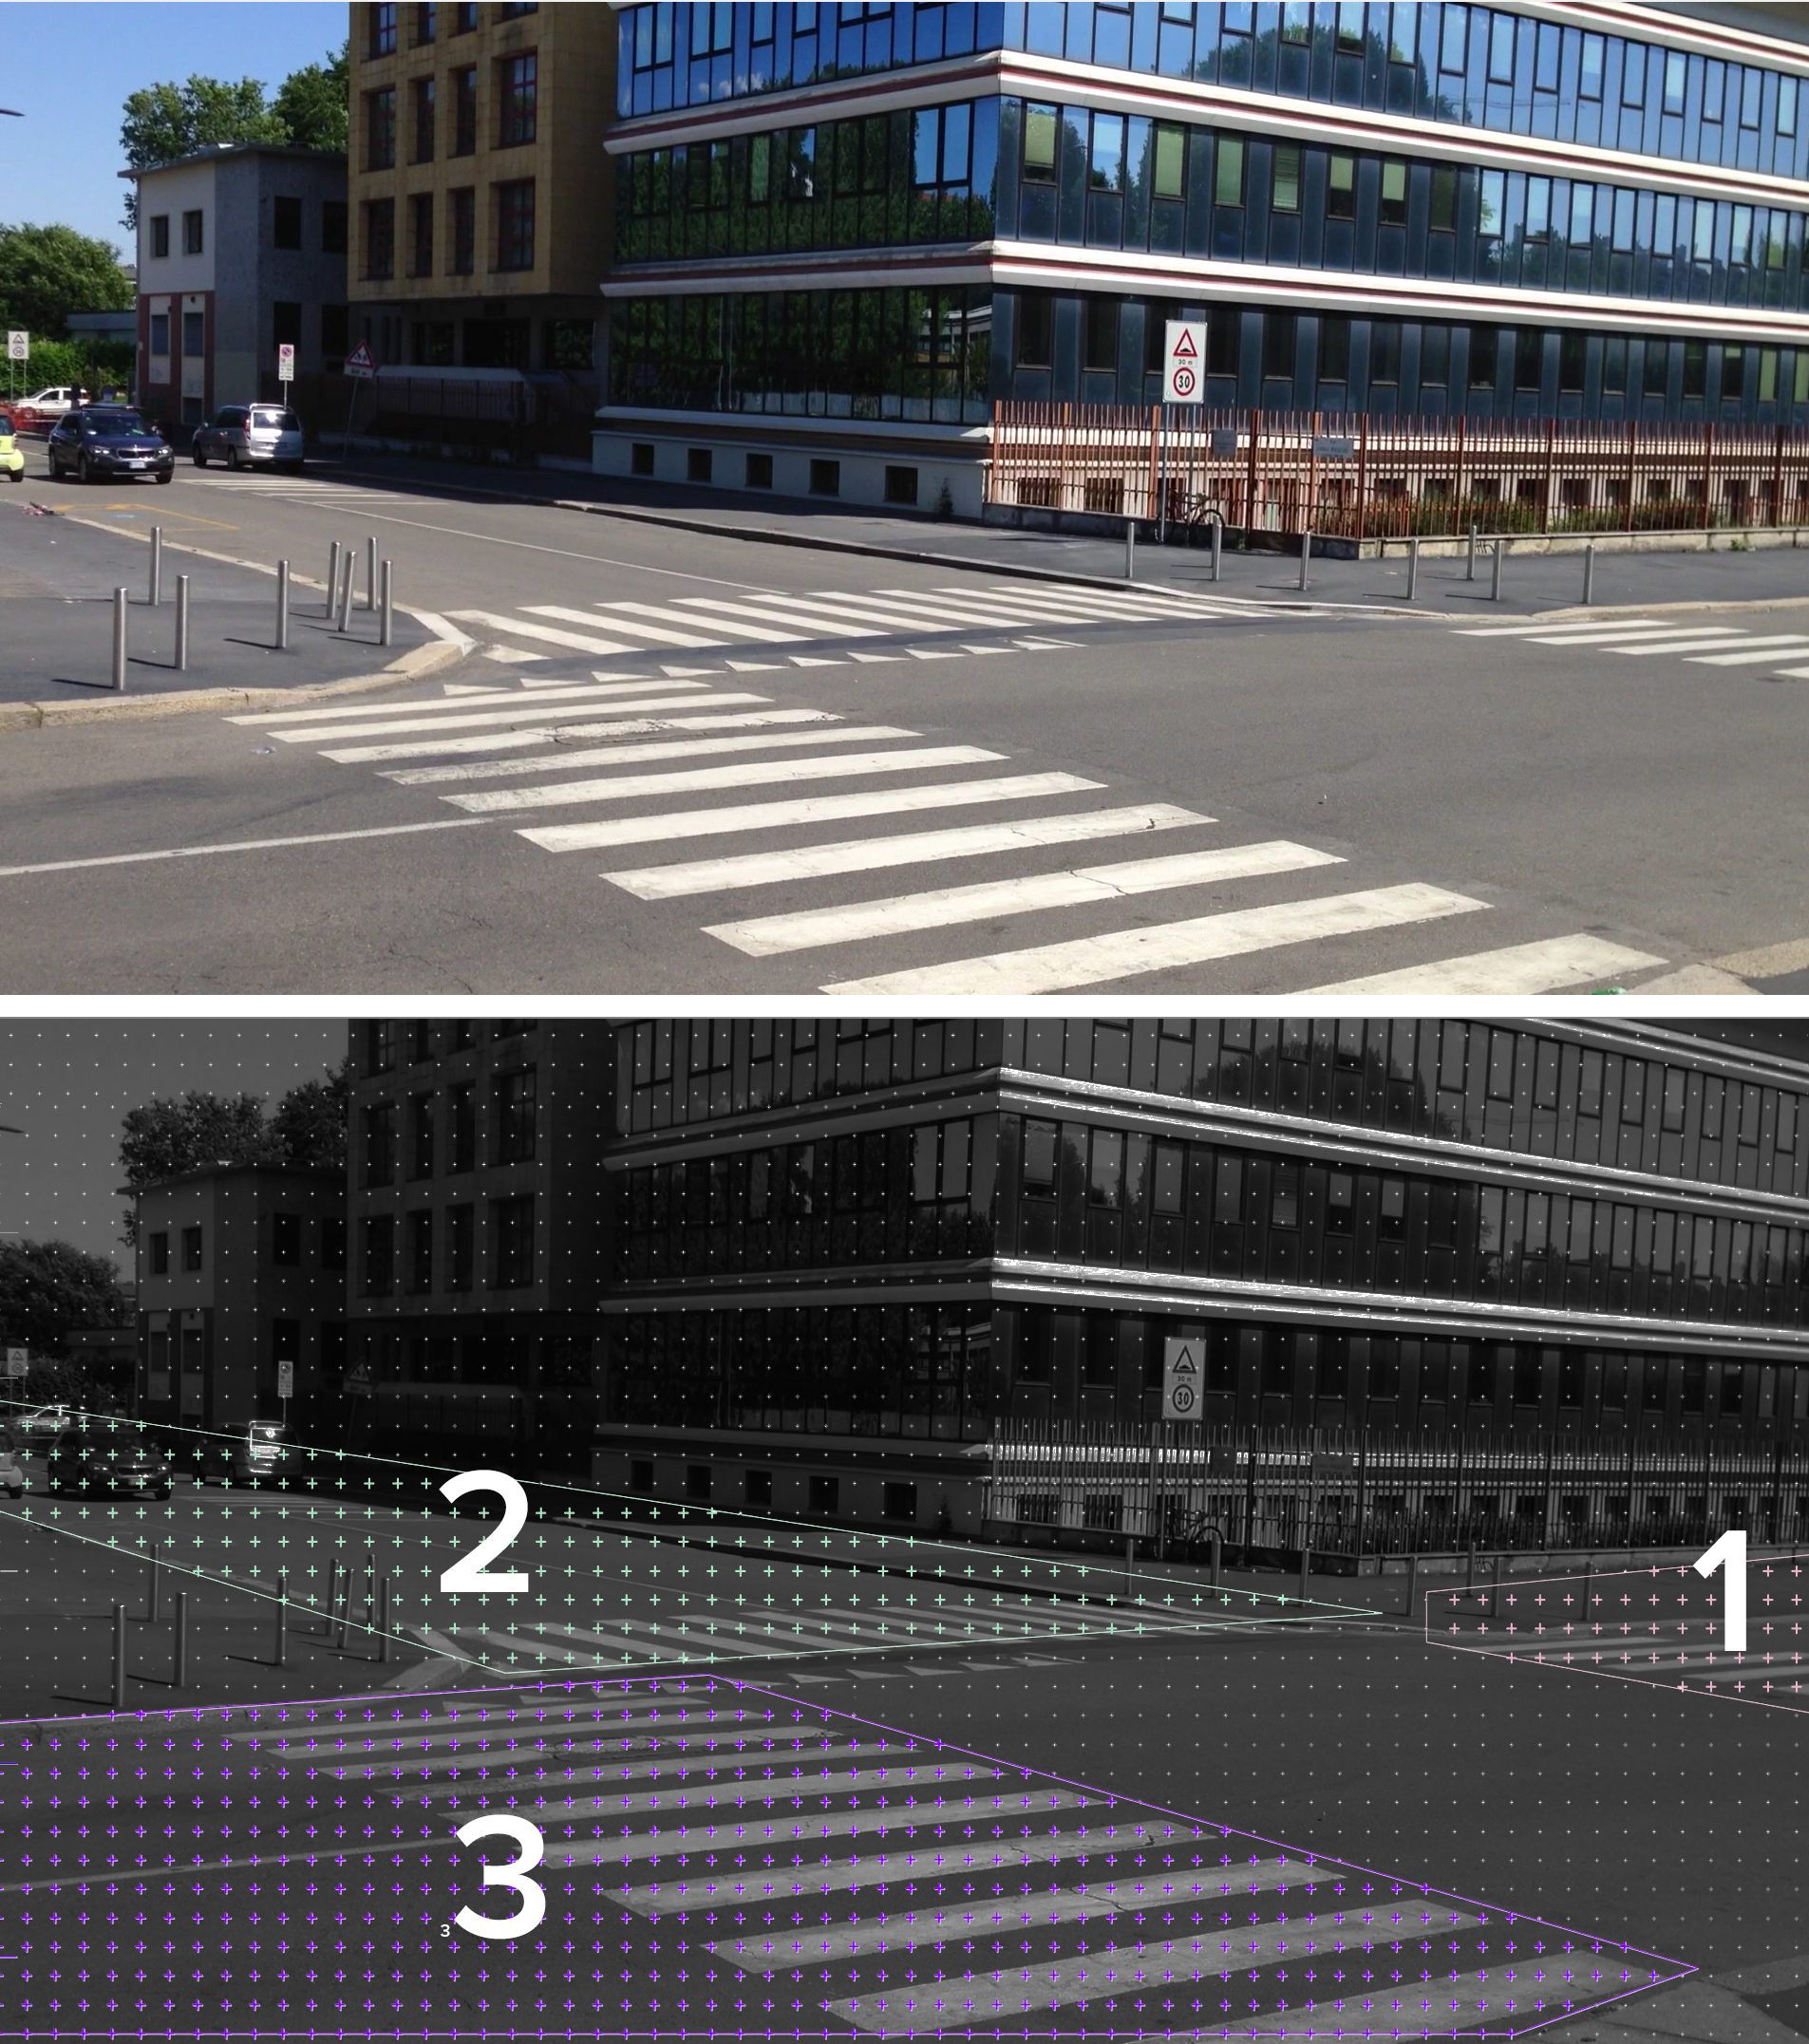
\includegraphics[width=0.8\textwidth]{images/priority_detection.jpg}
\caption{Detecting car's priority}
\label{fig:priorities}
\end{figure}

Having the system set up in this way, it's trivial to see that the only right-hand side rule violation could happen between cars of priority (1, 2) and  (2,3). 
Next we track the cars and in each frame check for possible traffic violation between those the priority pairs. This is is done within functions \textit{determineIfViolaitonP12} and \textit{determineIfViolaitonP23}. In order for the program to decide if a violation between cars with priority 1 and 2 has happened these conditions need to be satisfied:

\begin{itemize}
\item the distance between the left bounding box edge of vehicle with priority 2 and the one with priority 1 has to be greater than \textit{ minDeltaDist = 10}. Meaning we make sure the cars have passed each other

\item the distance between the top bounding box edge of vehicle with priority 1 and the one with priority 2 has to be greater than than \textit{ minDeltaDist = 10}. Meaning we make sure the car with priority 1 didn't make a left turn and is now "above" the car with priority 2

\item the overlap ratio of their bounding boxes has to be greater than \textit{ minOverlap = 0.2}.
\item the difference between velocity \footnotemark of the vehicle with priority 2 and the one with lower priority has to be greater than  \textit{ minDeltaVelocity = 250}. 
Meaning, the vehicle with the higher priority has to have a much lower velocity, as though it was stopping or slowing down
\end{itemize}
\footnotetext{The term velocity here is used somewhat loosely, because the true velocity could have been calculated only in case the actual intersection section dimensions were known, and if the center of the bounding box was less volatile. The calculation used for this velocity indicator can be found in the function \textit{updateVelocity}  }

\subsection{Manual}
The videos on which we have tested our software can be fond in the \textit{video\_data\_sunday} folder. 
The software can be run for any video by specifying its path with the \textit{videoPath} variable in the function \textit{main}.
Running it runs the the traffic detection violation program which outputs its result in the console. 

%----------------------------------------------------------------------------------------
%	CONCLUSION
%----------------------------------------------------------------------------------------

\section{Results} % Major section
The results obtained after testing each video are the following:
\begin{itemize}
 \item  \textit{video\_data\_sunday/IMG\_5108.mov} the software correctly decides the first encounter of vehicles with priority 1,2 is not a violation due to their overlap ratio not being sufficiently large. Furthermore, it also correctly decides the second encounter was indeed a violation
 \item  \textit{video\_data\_sunday/IMG\_6914.mov} an example of a car with priority 2 respecting the right-hand side rule, and stopping to let the car with priority 3 pass. The software correctly handles this situation 
 \item  \textit{video\_data\_sunday/IMG\_6915\_01.mov} an example of traffic violation between two motorcycles with priority 1 and 3 which the software detects correctly 
 \item  \textit{video\_data\_sunday/IMG\_6917.mov} in this video, the first car with priority 1 makes a left turn and the software correctly decides it is not a violation. But when a second car with priority 1 passes the car with priority 2 making it a violation, the bounding box unexpectedly "jumps" from the first to the second car, and they end up with each others priorities. As a result, the software doesn't detect the violation
 \item  \textit{video\_data\_sunday/IMG\_6919.mov} An example of one non-violation between (1,2) and one violation between (1,2) which software correctly detects
\end{itemize}


Unfortunately, because of the conditions regarding video recording, we weren't able to procure a video where a violation of the right-hand side rule between vehicles with priority 2 and 3 had happened. Hence we were not fully able to test it for that particular instance.
In addition, we feel obligated to point out that even the slightest shake of a camera can cause the surrounding background to be detected as a moving object, which consequentially renders the software useless in traffic violation detection. 
Furthermore, all the videos we have tested are quite simple cases without much noise like pedestrians or too much traffic at the same time. In the future, it would be recommended to further refine motion detection so it also handles even more complex cases.

\clearpage
%----------------------------------------------------------------------------------------
%	BIBLIOGRAPHY
%----------------------------------------------------------------------------------------

\begin{thebibliography}{99} % Bibliography - this is intentionally simple in this template

\bibitem[Figueredo and Wolf, 2009]{Figueredo:2009dg}
Figueredo, A.~J. and Wolf, P. S.~A. (2009).
\newblock Assortative pairing and life history strategy - a cross-cultural
  study.
\newblock {\em Human Nature}, 20:317--330.
 
\end{thebibliography}

%----------------------------------------------------------------------------------------

\end{document}